\documentclass[14pt]{extreport}
\usepackage{cmap}
\usepackage[utf8]{inputenc}
\usepackage[english,ukrainian]{babel}
\usepackage{graphicx}
\usepackage{geometry}
\usepackage{listings}
\usepackage{amsmath}
\usepackage{float}
\geometry{
	a4paper,
	left=20mm,
	right=20mm,
	top=20mm,
	bottom=20mm
}
\lstset{
	language=bash,
	tabsize=4,
	breaklines,
	keepspaces,
	showstringspaces=false,
}
\graphicspath{ {./pictures} }
\setlength{\parindent}{4em}

\newcommand\subject{Конструювання програмного забезпечення}
\newcommand\lecturer{доцент кафедри ПЗ\\Сердюк П.В.}
\newcommand\teacher{доцент кафедри ПЗ\\Сердюк П.В.}
\newcommand\mygroup{ПЗ-32}
\newcommand\lab{2}
\newcommand\theme{ADO.Net ORM. Data access through ADO.Net EF}
\newcommand\purpose{Ознайомлення з засобами розробки ADO.Net ORM. Data access through ADO.Net EF}

\begin{document}
\begin{normalsize}
	\begin{titlepage}
		\thispagestyle{empty}
		\begin{center}
			\textbf{МІНІСТЕРСТВО ОСВІТИ І НАУКИ УКРАЇНИ\\
				НАЦІОНАЛЬНИЙ УНІВЕРСИТЕТ "ЛЬВІВСЬКА ПОЛІТЕХНІКА"}
		\end{center}
		\begin{flushright}
			Інститут \textbf{КНІТ}\\
			Кафедра \textbf{ПЗ}
		\end{flushright}
		\vspace{200pt}
		\begin{center}
			\textbf{ЗВІТ}\\
			\vspace{10pt}
			До лабораторної роботи № \lab\\
			\textbf{На тему}: “\textit{\theme}”\\
			\textbf{З дисципліни}: “\subject”
		\end{center}
		\vspace{40pt}
		\begin{flushright}
			
			\textbf{Лектор}:\\
			\lecturer\\
			\vspace{10pt}
			\textbf{Виконав}:\\
			
			студент групи \mygroup\\
			Коваленко Д.М.\\
			\vspace{10pt}
			\textbf{Прийняв}:\\
			
			\teacher\\
			
			\vspace{28pt}
			«\rule{1cm}{0.15mm}» \rule{1.5cm}{0.15mm} 2023 р.\\
			$\sum$ = \rule{1cm}{0.15mm}……………\\
			
		\end{flushright}
		\vspace{\fill}
		\begin{center}
			\textbf{Львів — 2023}
		\end{center}
	\end{titlepage}
		
	\begin{description}
		\item[Тема.] \theme.
		\item[Мета.] \purpose.
	\end{description}

	\section*{Лабораторне завдання}
	Відповідно до варіанту проекту з баз даних 
	\begin{enumerate}
		\item вивести на UI дані із таблиць. Дані вибирати відповідно до списку сценаріїв та планованого графічного інтерфейсу  
		\item Реалізувати додавання, оновлення та видалення даних за допомогою фреймворків ADO.Net EF 
		\item Реалізувати підходи DB First та Code First
		\item Реалізувати міграцію для Code First. Для цього змінити модель і згенерувати міграцію 
	\end{enumerate}
	
	
	\section*{Хід роботи}
	
	\begin{small}
		\begin{lstlisting}
		\end{lstlisting}
	\end{small}
	
	\begin{figure}[H]
		\centering
		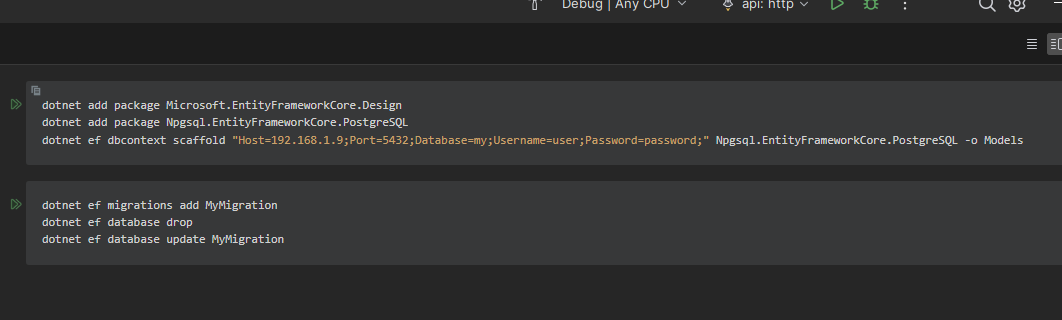
\includegraphics[scale=0.63]{1}
		\caption{В результаті виконання наступних команд}
	\end{figure}
	
	
	\begin{figure}[H]
		\centering
		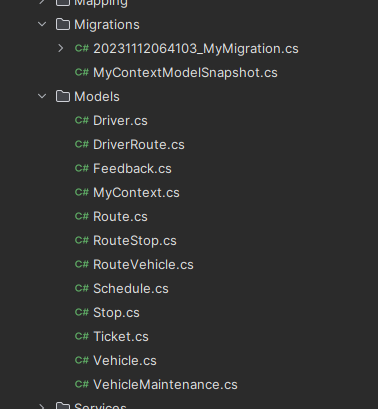
\includegraphics[scale=1]{2}
		\caption{Отримані моделі Db-first та міграції}
	\end{figure}
	
	\section*{Висновок}
	Під час виконання лабораторної роботи, я реалізував власний алгоритм руху роботів, з допомогою якого вони зможуть рухатися, колекціонувати енергію та створювати нових, а також розробив Unit-тести для перевірки роботи цього алгоритму.
	
	 
\end{normalsize}
\end{document}
